\section{Experiment 9F: control-aware personalized LPV manifold}
\label{sec:experiment9f}

\paragraph{Question and representation.}
Experiment 9E shows that exact family averaging cannot remove the Local gap,
because control-relevant within-family variation is genuine. Experiment 9F asks
whether that variation nevertheless lies on a low-dimensional manifold. In
log-parameter coordinates $z_i=\log\theta_i$, the personalized model is
\begin{equation}
 z_i=\mu_g+U_g a_i,
 \qquad \theta_i=\exp(z_i),
 \label{eq:personalized-manifold}
\end{equation}
where the group center $\mu_g$ and directions $U_g$ are shared, while
$a_i\in\mathbb{R}^r$ is retained by client $i$. Rank zero is the shared family
model, rank one gives a scalar local head, and rank three is the unreduced
three-parameter model.

Two bases are learned from 180 training clients per fresh fleet. Parameter-PCA
uses Euclidean variation in $z$. Control-PCA instead applies PCA after whitening
by
\begin{equation}
 W_g=\frac{1}{n_K}J_g^\top J_g+\eta I,
 \qquad
 J_g=\left.\frac{\partial\operatorname{vec}K(v,\exp z)}{\partial z}
 \right|_{z=\mu_g},
 \label{eq:control-metric}
\end{equation}
where scheduled LQI gains are sampled at five speeds and each gain output is
scaled by its root-mean-square sensitivity. This makes the first retained
direction preserve variations that most change the controller rather than
those that are merely largest in parameter space.

The bases are evaluated on 30 unseen clients for each of seeds 156--165 and on
the three held-out trajectories used in Experiment 9E. True family labels, true
training ratios, and oracle projections of the true test ratios are used. This
deliberate oracle protocol tests representation capacity only; it does not yet
claim that a client can estimate $a_i$ from finite data or that $U_g$ has been
learned by a federated protocol. The unchanged 9D Local fit is retained as the
practical comparator.

\begin{table}[htbp]
\centering
\caption{Experiment 9F unseen-client results. ``Gap closed'' measures recovery
from Exact-family toward Exact-individual.}
\label{tab:experiment9f-results}
\begin{tabular}{lrrrr}
\toprule
Method & Local dim. & Tracking & vs. Local & Gap closed\\
\midrule
Exact-family & 0 & 0.007522 & $+7.54\%$ & 0.0\%\\
Parameter rank 1 & 1 & 0.007468 & $+6.77\%$ & 6.6\%\\
Control rank 1 & 1 & 0.006952 & $-0.62\%$ & 69.5\%\\
Parameter rank 2 & 2 & 0.006704 & $-4.15\%$ & 99.6\%\\
Control rank 2 & 2 & 0.006720 & $-3.93\%$ & 97.7\%\\
Local fit & 3 & 0.006995 & --- & 64.2\%\\
Exact-individual & 3 & 0.006701 & $-4.20\%$ & 100.0\%\\
\bottomrule
\end{tabular}
\end{table}

\begin{figure}[htbp]
\centering
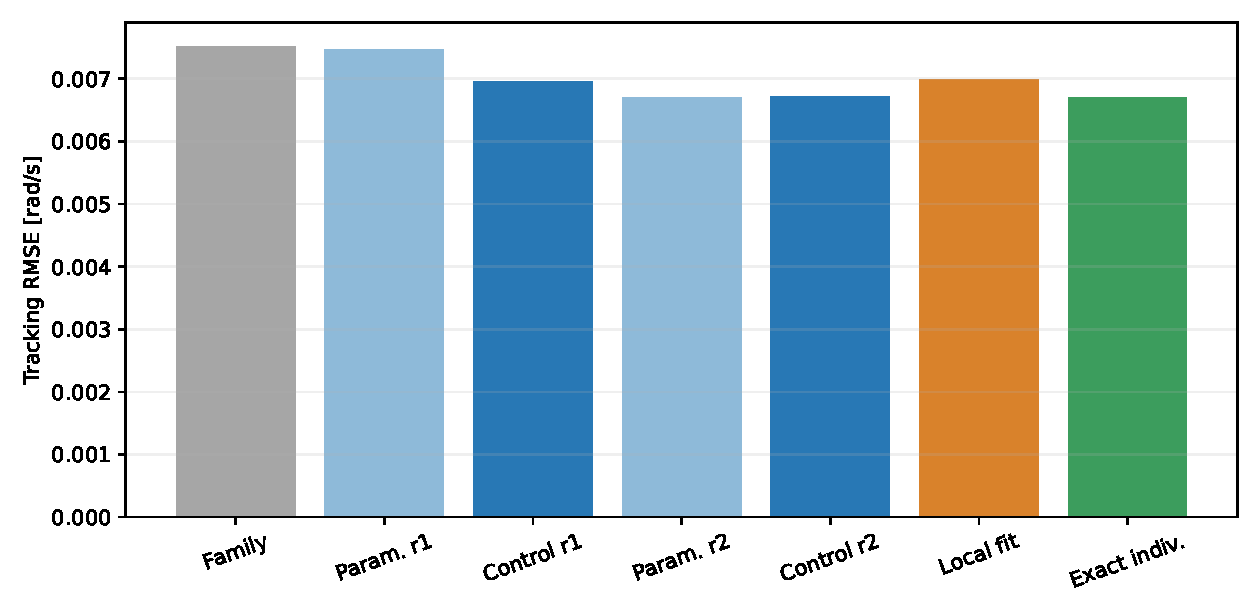
\includegraphics[width=0.84\linewidth]{../results/figures/experiment_9f_personalized_manifold.pdf}
\caption{Tracking as local personalization rank increases. Control awareness is
decisive at rank one; two coordinates are sufficient for either basis.}
\label{fig:experiment9f}
\end{figure}

\paragraph{Results.}
The rank-one outcome confirms the central hypothesis. Parameter-PCA reduces
parameter error but closes only 6.6\% of the control-performance gap and loses
to Local in all ten fleets. Control-PCA rank one closes 69.5\%, improves the
fresh-fleet mean over Local by 0.62\%, and beats Local in six of ten fleets. It
therefore provides mean parity rather than uniform superiority, but does so with
one client-specific scalar instead of a full three-parameter local model.

At rank two, both constructions recover essentially all useful individual
behavior. Control rank two is only 0.28\% above Exact-individual, closes 97.7\%
of the gap, and beats fitted Local in every fleet. Parameter rank two is 0.05\%
above Exact-individual and closes 99.6\%. Its slight advantage over the
control-aware version shows that the local quadratic gain metric is most useful
for ordering the first direction, not universally optimal at every rank.
Rank-three reconstruction error is $2.24\times10^{-16}$, and both bases exactly
recover Exact-individual as required. All 300 Local fits converge and all 8100
nonlinear evaluations are feasible.

The representation changes the deployment accounting. Per family, rank one
shares a three-parameter center and one three-element direction, while each
vehicle stores one coordinate. Rank two shares nine scalars per family and
retains two per vehicle. This is not a reduction in the number of personalized
controllers actually executed: each client still obtains a distinct gain
schedule. It is a reduction in client-specific model dimension and a structured
way to transfer population information.

\paragraph{Decision and next gate.}
Both predeclared structural gates pass: Control rank one is no worse than Local
on the fleet mean, and Control rank two lies within 1\% of Exact-individual with
fewer than three local coordinates. Personalized FL is therefore a reasonable
direction, but Experiment 9F alone is not yet an FL result. The next experiment
must learn $\mu_g$ and $U_g$ from client messages and estimate $a_i$ directly
from the same finite local records. It must compare calibration time as well as
tracking, because obtaining an oracle coefficient from the true test parameter
vector would otherwise hide the original identification problem.

A defensible personalized protocol alternates local scalar or two-coordinate
output-error updates with server aggregation of centers and basis directions.
Unknown groups can use the already validated uncertainty-aware soft membership.
The primary gate should require rank-one or rank-two personalization to retain
its advantage under finite-data coefficient estimation; privacy can then be
applied only to the shared updates, while $a_i$ remains on the vehicle.

\paragraph{Reproducibility.}
The frozen protocol is in \path{code/config/experiment_9f.json}; its implementation
is \path{code/experiments/experiment_9f_personalized_manifold.py}. Aggregate and
seed-level results, learned-basis summaries, comparisons, and provenance hashes
are stored under \path{results/tables}.
